% Copyright 2014 Yoshida Shin
% 
% This is part of "Git Second Step."
% 
% This program is free software: you can redistribute it and/or modify
%     it under the terms of the GNU General Public License as published by
%     the Free Software Foundation, either version 3 of the License, or
%     (at your option) any later version.
% 
%     This program is distributed in the hope that it will be useful,
%     but WITHOUT ANY WARRANTY; without even the implied warranty of
%     MERCHANTABILITY or FITNESS FOR A PARTICULAR PURPOSE.  See the
%     GNU General Public License for more details.
% 
%     You should have received a copy of the GNU General Public License
%     along with this program.  If not, see <http://www.gnu.org/licenses/>.

\begin{frame}{}{}
  もう一度 git add
\end{frame}


\begin{frame}[t]{もう一度 git add}{}
  \begin{columns}

    \begin{narrowcolumn}
      \begin{center}
        HEAD
        \vspace{2ex}

        
\begin{tikzpicture} [x=1em, y=1ex]
          \draw (0,0) rectangle (3,6);
          \draw (1.5,2) node {line1};
          \draw (1.5,4) node {line2};
        \end{tikzpicture}

      \end{center}
    \end{narrowcolumn}

    \begin{narrowcolumn}
      \begin{center}
        workspace
        \vspace{2ex}

        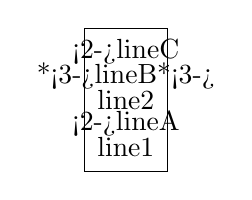
\begin{tikzpicture} [x=1em, y=1ex]
          \draw (0,0) rectangle (3,12);
          \draw (1.5,2) node {line1};
          \draw (1.5,4) node {\alert<2->{lineA}};
          \draw (1.5,6) node {line2};
          \draw (1.5,8) node {\onslide*<3->{\color{blue}}lineB\onslide*<3->{\color{black}}};
          \draw (1.5,10) node {\alert<2->{lineC}};
        \end{tikzpicture}

      \end{center}
    \end{narrowcolumn}

    \begin{narrowcolumn}
      \onslide*<5-8>{

        \code{
          diff {\dhyphen}git a/a b/a

          ...

          +lineC

          \onslide*<-6>{+lineB}

          ~line2

          +lineA

          ~line1

        }
      }

      \onslide*<11->{
      \begin{center}
        cached
        \vspace{2ex}

        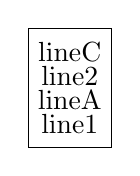
\begin{tikzpicture} [x=1em, y=1ex]
          \draw (0,0) rectangle (3,10);
          \draw (1.5,2) node {line1};
          \draw (1.5,4) node {lineA};
          \draw (1.5,6) node {line2};
          \draw (1.5,8) node {lineC};
        \end{tikzpicture}

      \end{center}

      }
    \end{narrowcolumn}

  \end{columns}
  \vspace{2ex}

  \onslide*<1>{
    調子に乗って、一度に一つのファイルを

    更新しすぎた

    2個の commit に分けたい
  }
  \onslide*<2-3>{
    \alert{この行だけ}次の commit で追加したい
    \vspace{2ex}

    \onslide*<3->{
      \color{blue}この行\color{black}はまた後で commit するので

      workspace で削除したくない
    }
  }
  \onslide*<4>{\$ git add -e \textit{path}}
  \onslide*<5>{エディタでパッチ編集画面が開く}
  \onslide*<6-7>{+lineB の行を消す}
  \onslide*<8-9>{エディタ終了}
  \onslide*<10-11>{
    HEAD のファイルに、

    先ほど編集したパッチを適用した物が

    cached に追加される
  }
  \onslide*<12>{
    この状態で commit すれば、

    workspace の更新を repository に部分適用可能
  }

  \onslide*<13>{
    commit の大きさは程度の問題であり、色々な方針が有ると思うが

    個人的には小さい commit 大好き
  }

  \onslide*<14>{小さい commit は小さい add に宿る}
\end{frame}
